\chapter{Introduction}\label{intro}

\section{The Interstellar Medium} 

The interstellar medium (ISM) is the material that fills the space between the stars in galaxies and is composed of cosmic rays, magnetic field lines, dust, and gas.  Each one of these constituents plays a role in shaping the overall physical and chemical behavior of a galaxy \citep{ferriere2001}.  This material is inhomogeneously spread about the galaxy's disk with dust and gas densities ranging from 1 particle per a thousand cubic centimeters to millions of particles per cubic centimeter (10$^{6}\geq$N$\leq$10$^{-3}$), and temperatures ranging from 10 K in the most dense regions to 10$^6$ K in the most diffuse \citep{ferriere2001}.  The constituents of the ISM will interact leading to the creation of molecular gas in giant molecular clouds (GMCs) and eventually to the formation of stars \citep{field1965}.  After the stars are formed, they will eject new material back into the ISM through stellar winds and supernovae repopulating the ISM, where each successive iteration introduces heavier atoms creating a galactic ecosystem \citep{ferriere2001}.  In this thesis we focus on the physical properties of the dust component of the ISM of the nearby barred spiral galaxy NGC3627 and also use the dust properties to learn more about its molecular gas properties.

\subsection{GMC Formation}

Intergalactic gas can be accreted into a host galaxy where it will condense and lead to the formation of molecular clouds \citep{kennicutt2012}.  The dominant process of GMC formation is divided between two camps, either a ``bottom-up'' or ``top-down'' formation scenario \citep{mckee2007}.  The bottom-up scenario consists of small clouds of cold HI coagulating to eventually form a GMC \citep{field1965, kwan1979}.  The major concern with the bottom-up scenario is if we include heating mechanisms in the cloud, coagulation will cease before the observed masses are reached \citep{mckee2007}.  The amount of time to accumulate enough mass to form a relatviely small GMC of 10$^5$ M$_\odot$ would take around 10$^8$ years which is much greater than the expected lifetime of a GMC \citep{kwan1979}.

The alternative formation scenario, top-down, postulates that GMC formation comes from instabilities in the diffuse ISM causing the clouds to collapse from their surrounding medium \citep{mckee2007}.  Two main instabilities are thought to be responsible for the collapse.  The first type of instability is a Parker instability, which involves distortion of magnetic field lines in the mid-plane of the galaxy, and at the location of these distortions gas will begin to accumulate \citep{parker1966, dobbs2013}.  The second instability responsible for collapse can be determined by the amount of rotational shear present \citep{mckee2007}.  If a strong rotational shear is present, such as in the inter-arm region of a spiral galaxy, then the accumulation of gas will be due to its shearing as it moves through the disk of a galaxy in a process known as swing amplification \citep{mckee2007, dobbs2013}.  If no rotational shear is present, such as in the inner regions of a galaxy or spiral arms, then the collapse can be attributed to a magneto-Jeans instability which will remove the angular momentum responsible for the rotational shear through magnetic fields in order for the normal Jeans instability to occur \citep{elmegreen1987,kim2001}.

%so the rotational shear is due to the spiral arms rotating though the galaxy which will distrupt the standard jeans instability of balancing thermal pressure and gravity.  Essentially it is shearing the cloud. Where minimal rotational shear is present, the jeans instability can occur however it is furthur enhanced by a magneto jeans instability.  
\subsection{Molecular Hydrogen Formation}\label{h2form}

Regardless of either collapse or coagulation, molecular hydrogen is being formed inside the cloud.  Molecular hydrogen can be formed via the two body reaction, three body reaction, formation using a free electron or proton, or surface formation \citep{krumholz2014}.  The two body formation scenario is the simplest reaction using two hydrogen atoms to produce molecular hydrogen,

\begin{equation}\label{eq:2bod}
  \ce{H + H -> H_2}
\end{equation}

However, two body formation is not the major mechanism in the formation of H$_2$ due to the requirement of a forbidden photon that arises from the combination of hydrogen atoms in the ground state \citep{gould1963}.  If one of the hydrogen atoms is excited, the transition can occur and molecular hydrogen is formed, but the number of excited hydrogen atoms in the temperature ranges typical of the cold and warm phases of the ISM are expected to be nearly nonexistent \citep{krumholz2014}.

The second formation scenario listed, three body formation, involves three hydrogen atoms coming together to form molecular hydrogen with a spare hydrogen atom,

\begin{equation}\label{eq:3bod}
  \ce{3H -> H_2 + H}.
\end{equation}

The required density for three body formation to occur is on the order of 10$^8$ cm$^{-3}$ \citep{palla1983,abel1997}, while the typical GMC density is on the order of 300 cm$^{-3}$.  The disparity between these densities eliminates any possibility of this being the primary mechanism to form molecular hydrogen in galaxies today. 

An alternative to the two or three body reactions uses either an electron or proton to ionize the hydrogen forming either H$^-$ or H$_2^+$ \citep{krumholz2014}.  The chemical reaction involving an electron is shown in equation \ref{eq:eform}, and the equation utilizing a proton is shown in reaction \ref{eq:pform}
\begin{equation}\label{eq:eform}
  \begin{split}
    \ce{H + \it{e} -> H^- + \it{h\nu}} \\
    \ce{H^- + H -> H_2 + \it{e}}
  \end{split}
\end{equation}

\begin{equation}\label{eq:pform}
  \begin{split}
    \ce{H + H^+ -> H^+_2 + \it{h\nu}} \\
    \ce{H^+_2 + H -> H_2 + H^+}
  \end{split}
\end{equation}

The main limitation of the free electron/proton formation mechanism is an undersupply of free electrons and protons.  Typical Milky Way conditions show that regions wih a density $>$1 cm$^{-3}$ have free electron and proton densities $<$10$^{-4}$ cm$^{-3}$ \citep{wolfire2003}.  Secondly, the H$^-$ ion in equation \ref{eq:eform} is more likely to interact with a stray photon than an electron resulting in the ion returning to the atomic state \citep{glover2003}.  While we observe singly ionized hydrogen regions, HII regions, only a small fraction of the region will successfully produce molecular hydrogen.

While the free electron/proton formation method is suspected to be the primary H$_2$ catalyst in the early universe \citep{herbst2005}, at low redshifts the formation of molecular hydrogen on the surface of dust grains is the dominant formation mechanism \citep{krumholz2014}.  Surface formation of molecular hydrogen will occur when a hydrogen atom strikes a dust grain and successfully sticks to the grain.  The hydrogen will then interact with another hydrogen atom to form H$_2$ and be ejected from the dust particle after the reaction has occurred \citep{pirronello1997}.  The same process occurs on the dust grain as the two body formation in the gas phase, but  the dust grain will act as a medium to absorb the energy that would create the forbidden photon \citep{krumholz2014}.

%it would be a good idea to explain the requirements of the dust since not all dust can form H_2

With a dominant mechanism for molecular hydrogen formation, a reaction rate can be defined based on the cross section of the grain, $\Sigma_{gr}$, a striking probability dependent on the temperature of the observed dust, S(T), the probability of molecular hydrogen forming on the grain, $\upepsilon_{H_2}$, the density of free hydrogen in the GMC, n$_H$, and the density of hydrogen attached to the grain surface, n$_H{_0}$ \citep{krumholz2014}.  Scaling the product of these properteis with the integrated collisional probability of a Maxwellian gas, the reaction rate is determined to be

\begin{equation}\label{eq:reac_rate}
  \frac{dn_{H_2}}{dt} = \frac{1}{2}\left(\frac{8k_bT}{\pi m_H}\right)^\frac{1}{2}\Sigma_{gr}S\left(T\right)\upepsilon_{H_2}n_{H}n_{H_0}
\end{equation}

\noindent where k$_b$ is the Boltzmann constant, T is the temperature, and m$_H$ is the mass of the hydrogen atom.  Equation \ref{eq:reac_rate} is often simplified to 

\begin{equation}\label{eq:reac_rate_sm}
  \frac{dn_{H_2}}{dt} = \mathcal{R}_{gr}n_H n_{H_0}
\end{equation}

\noindent by introducing a variable known as the formation rate, $\mathcal{R}_{gr}$, that is constrained using the column densities of CI, CII, HI, H$_2$ \citep{krumholz2014}.  The column densities of CI and CII are used to determine a reaction rate by examining their ratios and the mechanisms that convert ions to atoms and atoms to ions.  The neutralization of CII involves its interaction with polycyclic aromatic hydrocarbons, and the ionization of C takes place by interacting with far-ultraviolet (FUV) photons \citep{wolfire2008}.  The FUV intensity will also dictate the amount of dissociation of H$_2$ into H, and by balancing the amount of CI and CII with the amount of H and H$_2$, the FUV intensity can be determined as well as the amount of H$_2$ being produced \citep{wolfire2008}.  Typical reaction rates for the Milky Way have been found to be $\mathcal{R}_{gr}$=3x10$^{-17}$cm$^3$s$^{-1}$ \citep{jura1975, gry2002, wolfire2008}.

\subsection{Dissociation of Molecular Hydrogen}\label{h2destroy}

When molecular hydrogen has formed, it is still susceptible to photodissociation from FUV photons.  The energy required for a single photon to break the bonds of molecular hydrogen is 14.5 eV \citep{krumholz2014}.  Conveniently, this is also enough energy to excite atomic hydrogen, so photodissociation using a single photon is highly unlikely due to the abundance of HI in the ISM \citep{krumholz2014}.  However, a photon with an energy of 11-13.6 eV will not be able to ionize atomic hydrogen, but will be able to excite molecular hydrogen to its first and second excitation levels, the Lyman and Werner bands, respectively.  The excited H$_2$ will eventually settle via photon emission to its ground state with a finite probability of returning to two hydrogen atoms rather than maintaining its molecular state \citep{krumholz2014}.

A dissociation rate, $\zeta_{diss}$, can be obtained by scaling the total excitation rate, $\zeta_{exc}$, by the fraction of excited hydrogen molecules that will settle to an atomic ground state \citep{krumholz2014}.  The total excitation rate is found by summing each individual excitation from the ground state e.g. $\zeta_{exc,0-1}$, $\zeta_{exc,0-2}$.  In the Milky Way's diffuse ISM, the interstellar radiation field is 6-9x10$^{-14}$ erg cm$^{-3}$ over the range of 6-13.6 eV resulting in $\zeta_{exc} \approx 3\times10^{-10}$s$^{-1}$ \citep{draine2011}.  The expected fraction of H$_2$ to dissociate is between 0.11 and 0.13 resulting in $\zeta_{diss}\approx4\times10^{-11}$s$^{-1}$\citep{draine2011}.
Equating the formation and dissociation rates and then solving for a molecular hydrogen to atomic hydrogen ratio gives

\begin{equation}\label{eq:fd_eq1}
  \begin{split}
    \zeta_{diss} n_{H_2} & = \mathcal{R}n_{H_0}n_H \\
    \frac{n_{H_2}}{n_H} & = \frac{\mathcal{R}n_{H_0}}{\zeta_{diss}} \\
                        & = 8\times10^{-6}\left(\frac{4\times10^{-11}s^{-1}}{\zeta_{diss}}\right)\left(\frac{n_{H_0}}{10cm^{-3}}\right)
  \end{split}
\end{equation}

\noindent \citep{krumholz2014}.  From equation \ref{eq:fd_eq1} we can see, in the diffuse medium, atomic hydrogen is far more abundant than molecular hydrogen, as expected.

However, as the density of the gas increases via collapse or coagulation, the optical depth will also increase, limiting the number of FUV photons able to penetrate into the core of the cloud, a process known as shielding which is the main factor in accelating H$_2$ production \citep{draine2011}.  This shielding will decrease the value of $\zeta_{diss}$ which will increase the n$_{H_2}$/n$_H$ ratio in equation \ref{eq:fd_eq1}.  The increase in the molecular to atomic hydrogen ratio signifies the accumulation of molecular gas reservoirs.  The molecular gas density will build up and lead to fragmentation within the cloud, and will eventually lead to star formation.  

\section{Determining the H$_2$ Abundance}

From the previous section, the formation of molecular hydrogen will result in the energy released during formation to be absorbed by a dust grain while the other methods resulted in the emission of a photon to account for the change in energy.  The absorption of energy by the dust grain as opposed to the energy being released through emission results in the formation of H$_2$ being a dark process (\S\ref{h2form}).  Furthermore, since the molecule is made of two hydrogen atoms, an its symmetry and low mass means it has no permanent dipole moment making low energy rotational transitions nonexistant \citep{bolatto2013,kennicutt2012}.  The high symmetry and low mass does not mean H$_2$ is unexcitable, but that the temperatures required to excite molecular hydrogen (T $\gtrsim$ 100K) are above the temperature of a typical GMC \citep{bolatto2013}.  Also the returning of H$_2$ to the ground state will more often than not result in the molecule separating into two hydrogen atoms (\S\ref{h2destroy}).  For our purposes, we can consider molecular hydrogen a dark molecule requiring special treatment to determine the amount present.

The amount of molecular hydrogen in a system can be calculated in several ways, and for the purpose of extragalactic sources they all involve using a molecular tracer to determine the amount of H$_2$ present.  The molecule most commonly used in extragalactic studies is CO due to its abundance and ability to be easily observed \citep{bolatto2013}.  Other tracers that have been used are CO's photodissociated counterpart, CII, in order to trace regions that have little to no CO emission \citep{madden1997}, and molecules such as OH that have been used in the past but have been limited to Milky Way targets due to difficulty in observing OH \citep{barrett1964}.  The amount of CO can then be converted to H$_2$ using a conversion factor given as either

\begin{equation}\label{eq:x}
  n_{H_2} = X_{CO} I_{CO}
\end{equation}

where n$_{H_2}$ is the column density, X$_{CO}$ is the conversion factor in units of cm$^{-2}$ (K km s$^-1$)$^-1$, and I$_{CO}$ is the CO intensity in units of K km s$^{-1}$.  Typical values for X$_{CO}$ in normal spiral galaxies tend to be around 1-4$\times 10^{20}$ cm$^{-2}$ (K km s$^{-1}$)$^{-1}$, and a commonly used value for the Milky Way is 2$\times 10^{20}$ cm$^{-2}$ (K km s$^{-1}$)$^{-1}$ \citep{bolatto2013}.  Alternatively, the conversion factor can be used to determine the surface density of the molecular hydrogen, $\Sigma_{H_2}$, using

\begin{equation}\label{eq:alpha}
  \Sigma_{H_2} = \alpha_{CO} I_{CO}
\end{equation}

where $\alpha_{CO}$ is given in units of M$_\odot$ pc$^{-2}$ (K km s$^{-1}$)$^{-1}$.   Values of $\alpha_{CO}$ for nearby extragalactic sources have shown a mean value of 3.1 M$_\odot$ pc$^{-2}$ (K km s$^{-1}$)$^{-1}$ which is slightly lower than the assumed Milky Way value of 4.4 M$_\odot$ pc$^{-2}$ (K km s$^{-1}$)$^{-1}$ \citep{sandstrom2013}.

\subsection{Methods for Determining CO-to-H$_2$ Conversion Factor}\label{gettinx}

Several methods are available to determine the conversion factor for extragalactic sources, and each has its own caveats.  One common method used to determine the conversion factor is to use the virial nature of GMCs \citep{bolatto2013}.  The virial nature of GMCs implies that the clouds are gravitationally bound and not collapsing due the balance of the temperature of the cloud and amount of material present and the prevention of collapse can be aided by magnetic support \citep{mckee2007}.  This method works best for well defined clouds; however in the case of more distant nearby galaxies, the issue of whether or not giant molecular associations (GMAs) display the same virialization as their constituent GMCs can limit concrete results \citep{bolatto2013}.  The second caveat to using the virial mass to determine the conversion factor is that the method will only trace CO bright regions.   Tracing only CO bright regions produces results that show no dependence between the conversation factor and metallicity, while other methods display a negative correlation between the conversion factor and metallicity  \citep{bolatto2013}.  The lack of correlation with metallicity is believed to be due to the level of dust shielding present in the system.  If the amount of dust present in the region is large, then the region will display a large metallicity, and if little to no dust is present, the region will show a low metallicity. Regions with low metallicity will correspond to regions with little to no dust resulting in poor shielding.  The lack of shielding will allow the CO to be dissociated resulting in large amounts of self sheilding molecular hydrogen traced by ionized and atomic carbon gas instead of CO \citep{bolatto2013}.  While the virial method is suitable for determining conversion factors within CO bright regions, excluding any low metallicity regions will underestimate the total amount of H$_2$ present in the system as well as skew any possible relations of the conversion factor with metallicity \citep{bolatto2013}.

A second method to determine the conversion factor is to incorporate observations of isotopologues of CO that are optically thin, commonly $^{13}$CO \citep{bolatto2013}.   The temperature, density, and column or surface density of $^{13}$CO can be used to constrain the physical conditions of the GMC or GMA being examined.  The main problem with using this method is the degeneracy between the temperature and density of CO emission such that hot low density regions can resemble cool dense regions \citep{rosenberg2014}. This method also shares the same problem as the virial technique in that it only probes CO bright regions of the target leaving any CO-faint H$_2$ gas untraced \citep{bolatto2013}.  The issue of CO-faint molecular hydrogen has been examined using the photodissociated tracer of CO, CII, instead of $^{13}$CO.  The CII ion was used as a tracer of molecular hydrogen in dwarf galaxies and revealed large reservoirs of self-shielding H$_2$\citep{madden1997}.

The third way to determine the CO-to-H$_2$ conversion factor is by incorporating the emission from dust to determine the amount of molecular gas present.  This method assumes that the gas is well mixed and has a constant ratio of dust mass to gas mass present in the galaxy \citep{leroy2011}, which has been shown to be true for the Milky Way \citep{boulanger1996}.  A suitable conversion factor is found by solving 

\begin{equation}\label{eq:aco_dgr}
  \begin{split}
    \delta_{GDR}\Sigma_{dust} & = \Sigma_{H_2} + \Sigma_{HI} \\
    						  & = \alpha_{CO} I_{CO} + \Sigma_{HI} 
  \end{split}
\end{equation}

\noindent where $\Sigma_{dust}$, $\Sigma_{H_2}$, and $\Sigma_{HI}$ are the respective surface densities in M$_\odot$ pc$^{-2}$, I$_{CO}$ is the CO line intensity, $\alpha_{CO}$ is the conversion factor in M$_\odot$ pc$^{-2}$ K$^{-1}$ km$^{-1}$ s, and $\delta_{GDR}$ is the total mass of the gas divided by the total mass of the dust known as the gas-to-dust ratio \citep{leroy2011,sandstrom2013}.  In equation \ref{eq:aco_dgr}, we can measure $\Sigma_{dust}$, $\Sigma_{HI}$, and I$_{CO}$ leaving only the conversion factor and gas-to-dust ratio free to vary.  An appropriate $\alpha_{CO}$ value will generate a molecular gas mass that produces a constant gas-to-dust ratio over the galaxy being studied. This method has been carried out extensively by \cite{sandstrom2013} on kpc scales on nearby galaxies as well as on both of the Magellanic clouds by \cite{leroy2011}.

Determining a conversion factor via the dust emission provides the capability to trace the CO faint regions of a target \citep{israel1997}.  Despite this advantage over the other two methods, using equation \ref{eq:aco_dgr} leaves any gas not associated with atomic hydrogen to be treated as H$_2$.  This is shown in equation \ref{eq:aco_dgr} given that the total amount of gas, is $\alpha_{CO}$I$_{CO}$ + $\Sigma_{HI}$, so any gas not associated with atomic hydrogen is assumed to be molecular hydrogen.  This means that the calculated amount of H$_2$ will include contributions from CO, OH, and CII as well as any other chemical species present in the region.  This will effectively increase the conversion factor and the overall amount of molecular hydrogen reported \citep{bolatto2013}, but given the dominance of H$_2$ in the dense regions of the ISM, any increase will be negligible.  Another caveat of this method rests with the assumption of a constant dust-to-gas ratio \citep{bolatto2013}.  Issues such as the gas-to-dust ratio's dependence on metallicity \citep{draine2007} can render this assumption null if not treated properly.  Nevertheless, the agreement of conversion factors between the dust based method and other methods used for more local targets suggests that any gas present that has been incorrectly assumed to be H$_2$ and local fluctuations in the metallicity of the target galaxy have very little effect on the final results \citep{bolatto2013}.

\section{Determining Dust Mass}

Calculating a conversion factor using dust emission requires a knowledge of the amount of dust present in our system to determine a gas-to-dust ratio.  Given that a significant portion of the dust mass lies within the cold phase we can calculate a dust mass using a modified blackbody fit over the cold portion of the dust's spectral energy distribution (SED) \citep{galametz2012}.  A slight modification needs to be introduced to our blackbody resulting in what is known as a greybody or modified blackbody (MBB).  The modification is necessary because the dust does not absorb and re-emit all of the light incident on its surface.  If we assume an isolated optically thin medium ($\tau_\nu \ll$1) with a blackbody source function, B$_\nu$(T), the radiative transfer equation can be written as 

\begin{equation}\label{eq:mbb_rad_t}
  I_\nu = \left(1-e^{-\tau}\right)B_\nu\left(T\right),
\end{equation}

\noindent and simplified using a first order Taylor expansion with $\tau_\nu \ll$1 to get

\begin{equation}\label{eq:mbb_optd}
  I_\nu = \tau_\nu B_\nu\left(T\right)
\end{equation}

\noindent The optical depth can be expanded to incorporate the surface density of the dust, $\Sigma_{dust}$, as

\begin{equation}\label{eq:mbb_optd_def}
  \tau_\nu = \kappa_\nu \Sigma_{dust}
\end{equation}

\noindent such that the units on $\Sigma_{dust}$ are in kg m$^{-2}$ as opposed to M$_\odot$ pc$^{-2}$.  The dust emissivity cross-section per unit mass is represented by $\kappa_\nu$ and is often referred to as the opacity.  The opacity will reflect the chemical makeup and grain structure of the dust, but will not indicate the grain size \citep{planckXI2013}.  The behavior of the opacity has been well fit with a power law such that opacity shows a dependence on the frequency of the observed emission \citep{hildebrand1983}.  The opacity is typically written as 

\begin{equation}\label{eq:mbb_kapp}
  \kappa_\nu = \kappa_{\nu,0}\left(\frac{\nu}{\nu_0}\right)^\beta
\end{equation}

\noindent where $\nu_0$ is a reference frequency, $\kappa_{\nu,0}$ is a reference opacity based on the reference frequency, and $\beta$ is the dust emissivity index.  Values for $\kappa_\nu$ have been calculated for several models of varying dust compositions and can range from 0.2 to 2 m$^2$ kg$^{-1}$ over the wavelengths used to model the cold component (100$\mu$m--850$\mu$m)\citep{li2001}.  The emissivity index has commonly been fit between ranges of 1.0 to 2.0  suggested from laboratory experiments \citep{walcher2011}.  However, with the influx of Herschel data the ability to fill in the sub-millimeter portion of the SED between 100$\mu$m and 500$\mu$m has allowed the emissivity index to be determined based on observations, which have shown a range from 1 to 2.5 \citep{galametz2012}.  It should be noted that the lower limit of $\beta$=1 is a hard cutoff due to limits determined by the Kramers-Kronig relationship in the optically thin case \citep{li2005}, but in extreme instances when the dust becomes optically thick $\beta$\ will approach 0.

With the opacity well defined, substituting equation \ref{eq:mbb_kapp} into equation \ref{eq:mbb_optd_def} and then into the original equation for the specific intensity of our MBB, equation \ref{eq:mbb_optd}, gives the formula for the specific intensity of a greybody as

\begin{equation}\label{eq:mbb_specI}
  I_\nu=\Sigma_{dust}\kappa_{\nu,0}\left(\frac{\nu}{\nu_0}\right)^\beta B_\nu\left(T\right)
\end{equation}

\noindent  Since we measure the flux of our target, it is useful to convert from the specific intensity to the flux using 

\begin{equation}\label{eq:specI_to_flx}
  F_\nu = \pi I_\nu \left(\frac{r}{D}\right)^2
\end{equation}

\noindent given the target is a uniform sphere with radius, r, and distance, D \citep{rybicki1986}.  Substituting equation \ref{eq:specI_to_flx} into the greybody equation, \ref{eq:mbb_specI}, gives

\begin{equation}\label{eq:mbb_sd}
  S_\nu=\frac{\Sigma_{dust}\pi r^2}{D^2}\kappa_\nu\left(\frac{\nu}{\nu_0}\right)^\beta B_\nu\left(T\right).
\end{equation}

Converting from surface density to overall mass is done using the relationship between mass and surface density of M=$\Sigma*$Area where the target's projected area is $\pi$r$^2$.  This gives a final modified blackbody equation of 

\begin{equation}\label{eq:mbb_fin}
  S_\nu=\frac{M_{dust}}{D^2}\kappa_\nu\left(\frac{\nu}{\nu_0}\right)^\beta B_\nu\left(T\right).
\end{equation}

The dust mass can be solved from equation \ref{eq:mbb_fin} by fitting the dust mass, temperature, and possibly the emissivity index.  The fitted mass will act as a normalizing factor for the SED and correspond with the mass associated with the peak flux.  The fitted dust mass should be used cautiously due to a sensitivity in mass with temperature fluctuations \citep{draine2007}. An alternative to using the fitted mass is to isolate the mass from equation \ref{eq:mbb_fin} to get 

\begin{equation}\label{eq:mbb_mass}
  M_{dust} = \frac{S_\nu D^2}{\kappa_\nu B_\nu\left(T\right)}\left(\frac{\nu}{\nu_0}\right)^{-\beta}
\end{equation}

\noindent and use the parameters returned from fitting.  This equation is best used with a longer wavelength observation that will explore the Rayleigh-Jeans tail of the modified blackbody.  This portion of the SED will see less of a dependence on the mass and temperature fluctuations \citep{draine2007}.  The main concern with both methods to determine the mass arises from fitting both the temperature and dust emissivity index and their strong anti-correlation \citep{galametz2012,tabatabaei2014}.  A common method to help break the degeneracy is to fix the emissivity index to a reasonable value based upon the opacity model \citep{tabatabaei2014}.

\section{NGC 3627}

In this thesis, we are using the new SCUBA-2 instrumentation on the JCMT, which observes both 450$\mu$m and 850$\mu$m emission simultaneously.  Utilizing multiple 60 minute scans in high quality weather we can better constrain the emissivity index in our fits, as well as increase the resolution compared to previous work.  With these new observations from the NGLS, we can better fit an SED and determine a more reliable dust mass to explore the amount of molecular gas present.  To take full advantage of the benefits of SCUBA-2, we have selected the target NGC3627 for its relatively small angular size, pronounced spiral features, and relatively large flux.

NGC 3627 is the most prominent member of the interacting trio of galaxies called the Leo triplet (NGC 3623, NGC 3627,  and NGC3628).  An optical image is shown in Figure \ref{fig:ngc3627_opt} while the data we used can be seen in sections $\S$\ref{sc2_imgs} and $\S$\ref{ancillary}.  The interaction between NGC 3627 and NGC 3628 has been well documented via HI emission in the form of a large HI debris tail extending from NGC 3628 in the direction of NGC 3627 \citep{rots1978,haynes1979}.  The interaction between these galaxies has resulted in a high star formation rate of over 1.7 M$_\odot$ yr$^{-1}$ \citep{calzetti2010}, making NGC 3627 a prime candidate to study the current star forming conditions.  The morphology of NGC 3627 is that of a barred spiral (SABb) with an inclination of 60$\degree$ \citep{reuter1996} at a distance of 9.4 Mpc determined by Cepheid variable observations \citep{freedman2001}.  Furthermore, the strong spiral arm features of this galaxy are unique due to speculation that they are not contained within the plane of the galaxy \citep{dumke2011,soida2001}.  This interpretation is supported by magnetic field lines traced by dust polarization that do not trace the spiral structure in the southeastern bar end \citep{soida2001} and CO observation with bimodal emission features in velocity space over the southeastern bar end \citep{dumke2011}.

\begin{figure}
  \centering
  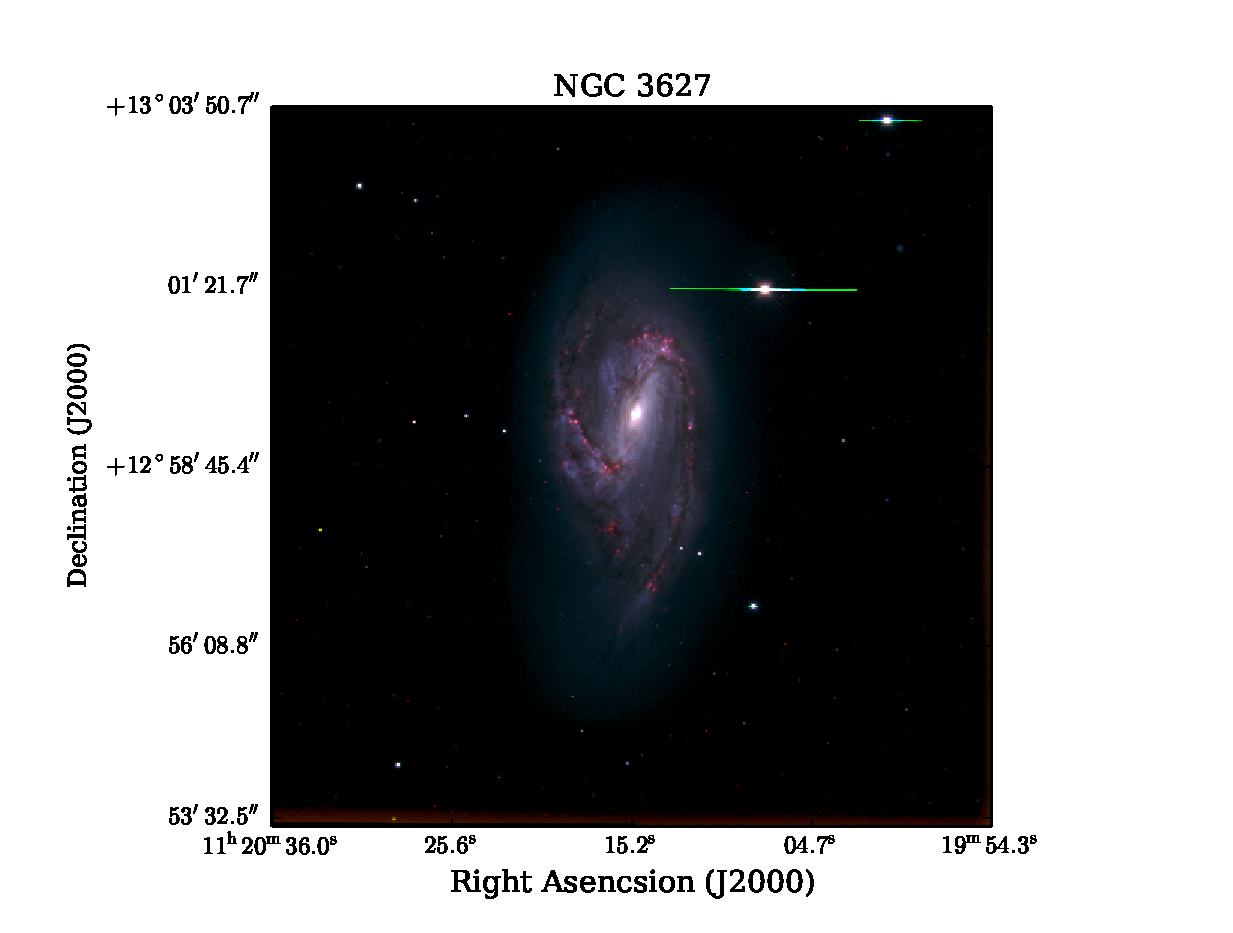
\includegraphics[width=1.\textwidth]{intro_imgs/rgb_tst.eps}
  \caption[Optical Image of NGC3627]{Optical composite image of NGC3627 made using the SINGS 5$^{th}$ enhanced data release \citep{kennicutt2003}.  Blue areas represent the B band, green areas represent V band and red areas show the H$\alpha$ band.  Component images were retrieved from NED.}
  \label{fig:ngc3627_opt}
\end{figure}

NGC 3627 was observed as part of the Spitzer Infrared Nearby Galaxies Survey (SINGS) \citep{kennicutt2003} and has been observed throughout the electromagnetic spectrum.  $^{13}$CO observations by \cite{watanabe2011} have shown that a majority of the star formation is occurring in the bar ends.  This information agrees with \cite{warren2010} showing the star formation efficiency being highest in the bar ends.  \cite{warren2010} also show the ISM of the galaxy to be dominated by molecular gas, with dense warm gas dominating the emission at the bar ends, the nucleus and a bright region located beneath the southwestern spiral arm, and more diffuse and cooler molecular gas outside of these regions.  The atomic gas is located primarily in the spiral arms with little to no emission in the nucleus of the galaxy.  A mean conversion factor of $\alpha_{CO}$=1.2 M$_\odot$ pc$^{-2}$ (K km s$^{-1}$)$^{-1}$ was found by \cite{sandstrom2013} using the dust method (\S\ref{gettinx}).  An HI mass was given as 8.18$\times$10$^8$ M$_\odot$ \citep{walter2008}, and a corresponding H$_2$ mass was calculated as 5.79$\times$10$^9$ M$_\odot$ \citep{kennicutt2003}, and a stellar mass of 2.8$\times$10$^{10}$ M$_\odot$ \citep{skibba2011}.

The dust emission of NGC 3627 follows the same trend as the CO emission with the brightest regions at the bar ends, nucleus, and a bright region below the southwest bar end.  The southeastern spiral arm shows some knotted features in the dust emission.  Global values for the cold and warm components of the SED were fit by \cite{galametz2012} and reveal dust temperatures of T$_W$=55.8$\pm$5.6 K and T$_C$=20.2$\pm$1.4 K for the warm and cold components, respectively, with a best fit emissivity index of $\beta$=2.3$\pm$0.2 and a total dust mass of 7.82$\times$10$^7$ M$_\odot$.

This thesis will explore the properties of dust emission from NGC3627 by exploring its SED using new observations from SCUBA-2 in order to measure the mass and dust emissivity index at a higher resolution in order to build on the work of \cite{galametz2012}.  Furthermore, we can use our SED derived dust masses to determine the overall amount of molecular gas present in the galaxy while gaining insight into the dust-to-gas ratio and conversion factor for this galaxy using the methods outlined by \cite{leroy2009} and \cite{sandstrom2013}.  The information in this thesis is arranged as follows: Chapter \ref{observations} will describe the data reduction and properties of the SCUBA-2 data and any ancillary data, Chapter 3 will describe the SED fitting method, Chapter 4 will include the results from the dust-to-gas ratio analysis, and Chapter 5 will summarize our findings.
